\section{Connectionist Temporal Classification (CTC)}

\begin{frame}[t,allowframebreaks]{Connectionist Temporal Classification (CTC)}
    \textbf{CTC: Solving the Alignment Problem in Sequence-to-Sequence Tasks}

    Many sequence tasks (e.g., speech-to-text) face the \textbf{alignment problem}: input and output sequences are of different lengths and not aligned. CTC enables training without explicit alignment.

    \begin{itemize}
        \item \textbf{Input:} Sequence $\mathbf{x} = (x_1, x_2, \ldots, x_T)$
        \item \textbf{Output:} Sequence $\mathbf{y} = (y_1, y_2, \ldots, y_U)$
        \item \textbf{Challenge:} $T \neq U$, unknown alignment
    \end{itemize}

    \textbf{CTC introduces a special \emph{blank} token ($\varnothing$) and allows repeated labels. The final output is obtained by collapsing repeats and removing blanks.}

    \begin{figure}[h!]
        \centering
        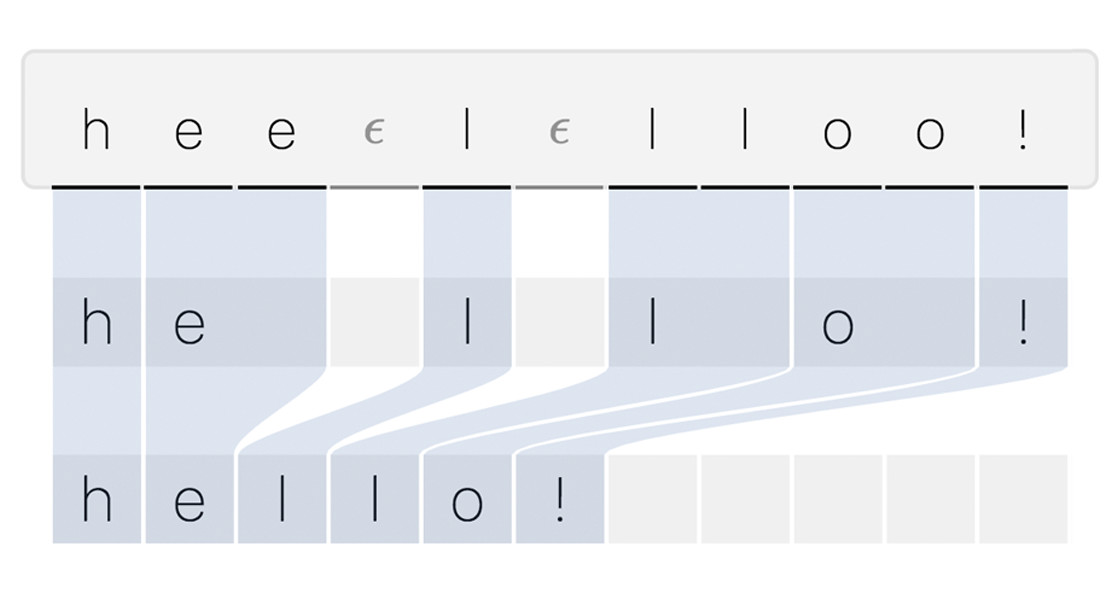
\includegraphics[width=0.8\textwidth]{images/audio-nlp/ctc.png}
        \caption*{CTC: Blank token insertion and collapsing.}
    \end{figure}

    \textbf{CTC Loss Function:}

    \begin{equation}
        L_{CTC} = -\ln \left( \sum_{\pi \in \mathcal{B}^{-1}(\mathbf{y})} \prod_{t=1}^{T} p(\pi_t | \mathbf{x}) \right)
    \end{equation}

    \begin{itemize}
        \item $\pi$: a possible alignment (path) with blanks and repeats
        \item $\mathcal{B}^{-1}(\mathbf{y})$: set of all paths that collapse to $\mathbf{y}$
        \item $p(\pi_t | \mathbf{x})$: probability of label $\pi_t$ at time $t$
    \end{itemize}

    \textbf{CTC Decoding:}
    \begin{enumerate}
        \item Predict a sequence of labels (including blanks) for each time step.
        \item Collapse repeated labels and remove blanks to get the final output.
    \end{enumerate}

    \begin{figure}
        \centering
        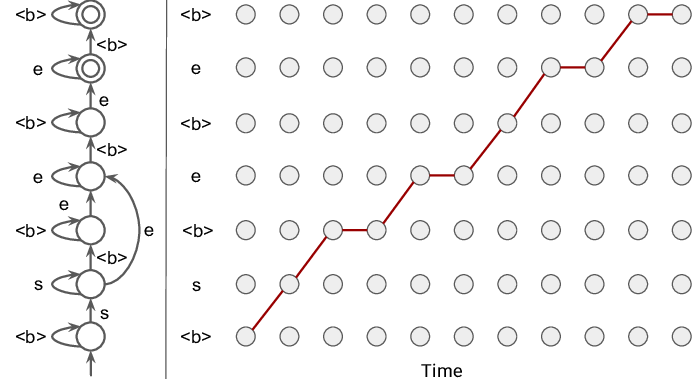
\includegraphics[width=0.9\textwidth]{images/audio-nlp/ctc-alignment.png}
        \caption*{CTC alignment: mapping input frames to output tokens via blank and repeat insertion.}
    \end{figure}
\end{frame}